%!TEX root = ../../thesis.tex

\chapter{Reassortment in Influenza Evolution}
\label{ch:influenza}

\section{Introduction}
\label{flu:introduction}

In this chapter we analyze influenza A virus, a common human pathogen.
Influenza is an enveloped single-stranded negative-sense RNA virus of family Orthomyxoviridae.


It is well known that frequent reassortment punctuates the evolution of influenza.
Reassortant strains can lead to antigenic novelty when internal segments adapted to humans pair up with novel external segments.
Indeed, such events led to the human influenza pandemics of 1957 and 1968.
Influenza provides a useful testbed for detection of reticulate evolution because of the large quantity of data that has been collected.

It is well-known that frequent reassortment of viral segments punctuates the evolution of influenza [cites].

Since the influenza pandemic of 2009, substantial effort has been put into.
The NCBI Influenza Virus Resource now contains over 400,000 unique viral isolates \cite{Bao:2008cq}.
The large quantity of genomic data that has been collected provides an ideal test bed for studying evolution in the reticulate limit.
Also because it allows for temporal analysis 

To test our model on biological data, we considered reassortment in avian influenza virus.
Influenza is a single-stranded RNA virus that is naturally found in avian populations.
Each viral genome has eight genetic segments.
Subtypes are defined by two segments, hemagglutinin (HA) and neuraminidase (NA), e.g. H1N1 and H3N2.
When a host cell is coinfected with two different viral strains, reassortment of these segments can occur, such that viral offspring is a genetic mixture of the two parental strains.
Reassortment is of substantial medical interest, and has been connected with the outbreak of influenza epidemics.

In fact, reassortment has been shown to be quite frequent even 

Natural host reservoir: aquatic birds.
Origin of 2009 H1N1 pandemic: triple reassortment.
Origin of 2013 H7N9 pandemic: triple reassortment.
Also discuss H5N1 and H5N2.

things we did:
applied PH to flu sequences
applied to segments individually -- no H1 homology
applied PH to concatenated sequences -- lots of higher homology
used to estimate recombination rates
looked at $H_1$ pairwise - determined that polymerase complex goes together.
[consistent with Greenbaum]

Important question: human adaptation
Pandemics: 1918 Spanish flu, 1957 Asian flu, 1968 Hong Kong, 2009 H1N1
Outbreaks: 2015 H5N2

Eight RNA segments that code for eleven proteins.
In recent years, there has been substantial concern over H5N1 and H7N9.
Total genome length approximately 13.5 kb

[from nelson 2007]
Host species barriers.
Pandemic potential.
Natural host reservoir.
 Wild waterfowl are the reservoir hosts for type A influenza viruses, harboring numerous antigenically distinct subtypes (serotypes) of the two main viral antigens, the haemagglutinin (HA) and neuraminidase (NA) sur- face glycoproteins (16 HA and 9 NA subtypes).

Include discussion of antigenic effects.
Combined effect of genetic drift and reassortment.

Experimental studies have shown that reassortment occurs at high frequency when segments do not mismatch \cite{Marshall:2013kn}.
This type of reassortment would be difficult to capture in our approach.

Rates of reassortment were first measured in \cite{Macken:2006jw}

\section{Influenza Virology}
\label{flu:virology}

Influenza has a segmented genome
Influenza is a single-stranded RNA virus of family Orthomyxoviridae.
Influenza has a segmented genome with eight segments coding for 11 proteins.
The segments are generally ordered from longest to shortest.

HA is the surface antigen that is responsible for binding the viral particle to the cell.
HA binds to sialic acid groups on the cell surface.
HA is the strongest determinant of host specificity: different hosts express different sialic acid types.
Avian influenza binds to type 2-3 sialic acid receptors, while human influenza binds to type 2-6 sialic acid receptors.
Human and avian adaptations.
NA is the surface protein that cleaves the replicating virus from the cell surface.
Together, HA and NA determine the subtype of virus and are a first marker of host transmission and specificity.

PB1, PB2, and PA form the polymerase complex and are involved in viral replication.
Mutations in these proteins can be among the most important in determining host adaptation and virulence.

The remaining proteins, including NP, M1, M2, and NS1 are largely structural proteins involved in capsid formation and viral packaging.

\begin{figure}
\begin{center}
\centerline{\includegraphics[width=.5\columnwidth]{./fig/influenza/flu_genome.jpg}}
\caption[Structure of an influenza virus particle]{Structure of an influenza virus particle. The surface capsid is formed from matrix proteins M1 and M2. Surface antigens HA and NA coat this surface and are involved in cell entry and exit. PB1, PB2, and PA form a polymerase complex assisting in }
\label{fig:flu:genome}
\end{center}
\end{figure}

Therefore, ways of automatically characterizing and representing reassortment are necessary.

We applied persistent homology to data for more than 3,000 avian influenza genomes from the NIH Influenza Sequence Database.
Examining each genome segment separately, we recovered only zero-dimensional homology, consistent with no intra-segmental recombination.
In other words, segment-by-segment the evolution of influenza is tree-like and amenable to a phylogenetic tree representation.

However, a similar analysis of the concatenated full genome reveals a complex topology, with a large number of loops in one and two dimensions.

\section{Influenza Reassortment}
\label{flu:reassortment}

The evolution of influenza is punctuated by frequent reassortment.
To characterize influenza evolution, we computed the persistent homology of four influenza datasets from avian, swine, and human hosts, each numbering as many as 1,000 genomic sequences.
When applied to a single segment of the virus unaffected by reassortment, higher-dimensional homology groups vanish (Fig. 2).
Alignments of single segments are therefore suitable for phylogenetic analysis.
In settings of vertical evolution, we can directly transform a filtration of 0-D simplicial complexes into an equivalent distance-based dendrogram.
Fig. 2A represents the zero-dimensional topology of the hemagglutinin segment of avian influenza viruses. 
The zero-dimensional generators at higher genetic distances indicate the major clusters, coinciding with the antigenic subtypes H1-H16.
From the bar sizes of the barcode plot, we can create a dendrogram that recapitulates classic phylogenetic analyses (Fig. 2B).
Only when segments are concatenated does persistent homology indicate that reassortment precludes phylogenetic analysis (Fig. 2C).
These results show that persistent homology can detect pervasive reassortment in influenza.
Estimating ICR from one-dimensional homology provides a lower-bound on reassortment rate in influenza.
We calculate an ICR of <1 event per year for classic H1N1 swine and H3N2 human influenza viruses, supported by previous phylogenetic estimates.
In contrast, we calculate a high reassortment rate of 22.16 events per year for avian influenza A.
This difference could be explained by the high diversity and frequent co-infection of avian viruses and correlates with the high proportion of potential avian reassortants reported in previous studies.

To illustrate how higher-dimensional topology captures reassortments, we analyzed 1,000 human H3N2 genomes and identified three generators of one-dimensional homology when joining the PB2 and HA segments.
As an example, the [G3] generator with the longest bar (Dataset S1, Table S5) is represented by an oriented one-dimensional irreducible cycle, implying at least one reassortment involving PB2 and HA of the isolates or their ancestors.
The number of sequences in the generator serves as an upper bound on the number of candidate reassortants.
Simple observation of the resulting sequence alignment reveals two divergent allelic patterns between informative sites in PB2 and HA, as reflected in incongruent trees (SI Appendix, Fig. S8 A and B) and reticulate cycles of the phylogenetic network (SI Appendix, Fig. S8C).

Our analysis of the concatenated H1N1pdm genome identified two nontrivial cycles, nominating candidate H1N1pdm reassortments in humans (Dataset S1, Table S6).
Given the greater homogeneity of H1N1pdm sequences due to increased sampling, the number of informative sites among [G2] sequences was too small to perform maximum likelihood phylogenetic analysis.
We therefore visually inspected informative sites, which suggested potential reassortment of two viral strains each contributing [PB2, M1, NS1] and [PB1, PA, HA] (SI Appendix, Fig. S9A).
Phylogenetic network analysis supports these incompatibilities (SI Appendix, Fig. S9B).

One-dimensional $\ICR$ provides a lower-bound estimate of reassortment rate (SI Appendix, Fig. S10B).
We calculate $\ICR < 1$ event per year for classic H1N1 swine and H3N2 human influenza, supported by previous phylogenetic estimates \cite{Lycett:2012fqa,Holmes:2005cia}.
In contrast, we calculate a high rate of 22.16 reassortments per year for avian influenza A (Dataset S1, Table S16).
This difference could be explained by the high diversity and frequent coinfection of avian viruses \cite{Lubeck:1979ws} and correlates with the high proportion of avian reassortants reported in previous studies \cite{Dugan:2008iba}.

% figure
\begin{figure}
\begin{center}
\centerline{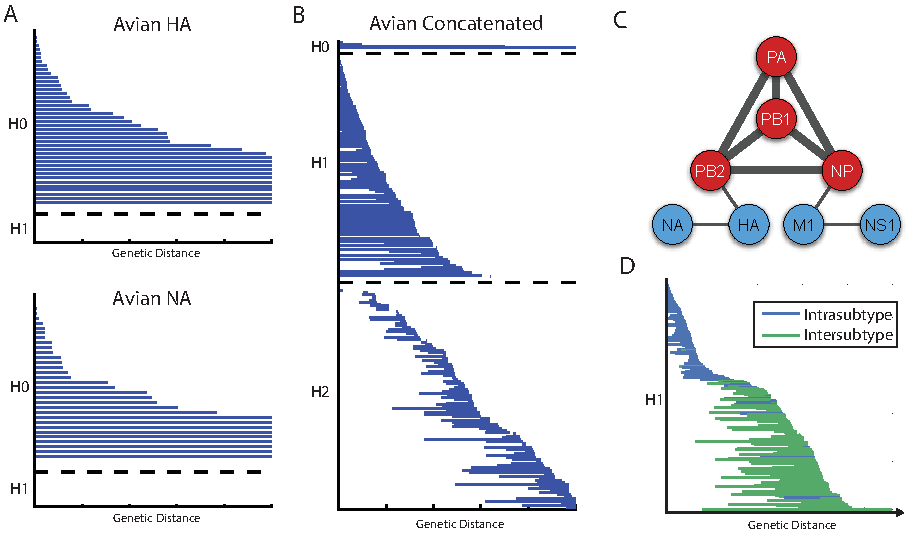
\includegraphics[width=\columnwidth]{./fig/influenza/influenza_Fig3.pdf}}
\caption[Influenza Megaplot]{Influenza Megaplot}
\label{fig:flu:megaplot}
\end{center}
\end{figure}

\section{Nonrandom Association of Genome Segments}
\label{flu:nonrandom_reassortment}

We observed nonrandom association of flu segments.
Statistical inference on the loops corresponding to reassortments identified segments that tend to co-segregate with each other during reassortment.In particular, polymerases co-segregate, while genes coding for envelope and capsid proteins show independent reassortment patterns.
Cosegregation of polymerases suggests that effective protein–protein interaction between the polymerase complex and the NP protein constrain reassortment. 

Although previous phylogenetic studies confirmed a high reassortment rate in avian influenza, none has identified a clear pattern of gene segment association \cite{Dugan:2008iba}.
To determine whether any segments cosegregate more than expected by chance, we applied persistent homology to avian influenza.
We first considered all pairs of concatenated segments and estimated the number of reassortments by $b1$.
We then ascertained the significance of observing a number of reassortments between each pair of segments given the total estimate of reassortments in the concatenated genome (SI Appendix, Supplementary Text).
Analysis of avian influenza reveals a statistically significant configuration of four cosegregating segments: polymerase basic 2 (PB2), polymerase basic 1 (PB1), polymerase acidic (PA), and nucleoprotein (NP) (Fig. 3D).
Interestingly, this pattern mimics previous in vitro results that suggest that effective protein-–protein interaction between the polymerase complex and the NP protein constrain reassortment \cite{Lubeck:1979ws}.

\section{Multiscale Flu Reassortment}
\label{flu:multiscale_reassortment}

We computed persistent homology on an aligned dataset of 3,105 avian influenza sequences across the seven major HA subtypes.
The persistence diagram is shown in Figure \ref{fig:flu:scatterplot}, along with density estimates for the birth and death distributions.
Both birth and death times appear strongly bimodal, unlike in the coalescent simulations, which were strictly unimodal.
This suggests two distinct scales of topological structure.
Using the representative cycles output by Dionysus on a subset of this data, we classified features as intrasubtype (involving one HA subtype) and intersubtype (involving multiple HA subtypes).
The $H_1$ barcode diagram for this data is shown in the Figure \ref{fig:flu:scatterplot} inset.
Intrasubtype features, in blue, occur at an earlier filtration scale than intersubtype features, in green.
The multiscale topological approach of persistent homology can distinguish biological events occuring at different genetic scales.

We isolated the two peaks and estimated two recombination rates: an intrasubtype $\rho_{1}=9.68$, and an intersubtype $\rho_{2}=21.43$.
We conclude that intersubtype recombination occurs at a rate over twice that of intrasubtype recombination, however a genetic barrier exists that maintains distinct subtype populations.
The nature of this barrier warrants further study.
This illustrates a real world example in which multiscale topological structure can be captured by persistent homology and given biological interpretation.

% figure
\begin{figure}
\begin{center}
\centerline{\includegraphics[width=\columnwidth]{./fig/influenza/flu_scatterplot.pdf}}
\caption[$H_1$ persistence diagram computed from an avian influenza dataset.]{The $H_1$ persistence diagram computed from an avian influenza dataset. On the top and left are plotted the marginal distributions of birth and death times, along with a density estimate for each distribution. The bimodality indicates two scales of topological structure. Inset: The barcode diagram for a subset of this data. Blue bars have representative cycles involving only one subtype, green bars have cycles involving multiple subtypes.}
\label{fig:flu:scatterplot}
\end{center}
\end{figure}

\section{Prediction of Host Specific Residues}
\label{flu:flumarker}

In this section, we describe work in prediction of host specific residues using machine learning approaches.
Host specific residues are important for viral surveillance in order to predict possible outbreaks.
We describe here two methods and include preliminary validation from our collaborator in Wisconsin.

\section{Conclusions}
\label{flu:conclusions}

The segmented nature of the influenza genome makes it an ideal 
Coinfection of a single cell by 
Coinfection of a single cell with multiple strains of influenza can lead to genomic reassortment.
Reassortments can lead to novel pandemics.
Therefore it is important that methods to characterize reassortment be developed.
In this chapter we have applied methods from TDA to characterize reassortment in influenza.
Using our approach, we have confirmed that intrasegmental recombination does not occur.
We have estimated reassortment rates.
We have estimated recombination rates.
Further, from the persistence diagram we identified a bimodal presence of $H_1$ invariants.
This suggests a genetic barrier maintaining subtype diversity.




